% Generated by code/needham.py -- do not edit by hand.
\definecolor{qocA}{rgb}{0.00,0.45,0.70}
\definecolor{qocB}{rgb}{0.90,0.60,0.00}
\definecolor{qocC}{rgb}{0.00,0.62,0.45}
\definecolor{qocD}{rgb}{0.80,0.40,0.00}
\definecolor{qocE}{rgb}{0.80,0.60,0.70}
\definecolor{qocF}{rgb}{0.35,0.70,0.90}
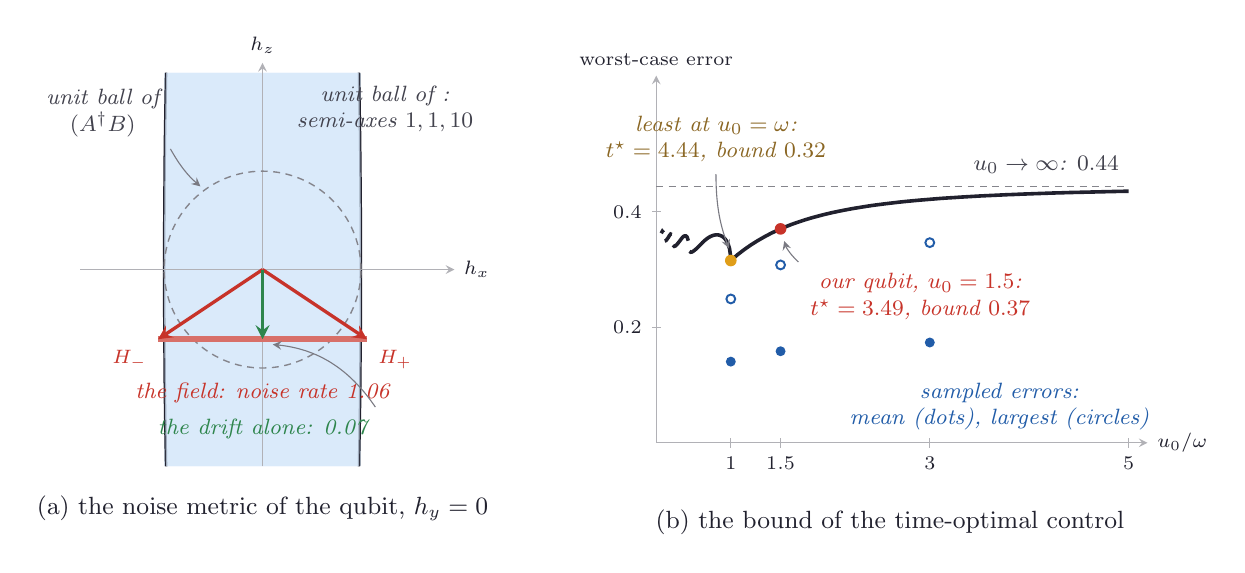
\begin{tikzpicture}[ink/.style={line width=0.9pt, ndInk}, faint/.style={line width=0.4pt, ndInk!35}, dashedink/.style={line width=0.5pt, ndInk!55, dash pattern=on 2.5pt off 2pt}, vec/.style={->, >=stealth, line width=1.2pt}, note/.style={font=\footnotesize\itshape, text=ndInk!85, align=center}, pointer/.style={->, >=stealth, line width=0.4pt, ndInk!60, shorten >=2pt, shorten <=1pt}, dot/.style={circle, fill=ndInk, inner sep=0pt, minimum size=3.4pt}, wash/.style={fill=ndSky, fill opacity=0.55}, every node/.style={text=ndInk}]
\definecolor{ndInk}{rgb}{0.13,0.13,0.18}
\definecolor{ndPaper}{rgb}{0.99,0.96,0.88}
\definecolor{ndSky}{rgb}{0.84,0.91,0.98}
\definecolor{ndRose}{rgb}{0.98,0.86,0.84}
\definecolor{ndBlue}{rgb}{0.13,0.36,0.66}
\definecolor{ndRed}{rgb}{0.78,0.20,0.16}
\definecolor{ndGold}{rgb}{0.88,0.62,0.10}
\definecolor{ndGreen}{rgb}{0.18,0.52,0.30}
\fill[ndSky, fill opacity=0.7] (1.350,0.200) rectangle (3.850,5.200);
\draw[ink] (3.825,0.200) -- (3.826,0.263) -- (3.827,0.325) -- (3.828,0.388) -- (3.830,0.450) -- (3.831,0.513) -- (3.832,0.575) -- (3.833,0.638) -- (3.834,0.700) -- (3.835,0.763) -- (3.836,0.825) -- (3.837,0.888) -- (3.838,0.950) -- (3.839,1.013) -- (3.839,1.075) -- (3.840,1.138) -- (3.841,1.200) -- (3.842,1.263) -- (3.842,1.325) -- (3.843,1.388) -- (3.844,1.450) -- (3.844,1.513) -- (3.845,1.575) -- (3.845,1.638) -- (3.846,1.700) -- (3.846,1.763) -- (3.847,1.825) -- (3.847,1.888) -- (3.848,1.950) -- (3.848,2.013) -- (3.848,2.075) -- (3.849,2.138) -- (3.849,2.200) -- (3.849,2.263) -- (3.849,2.325) -- (3.850,2.388) -- (3.850,2.450) -- (3.850,2.513) -- (3.850,2.575) -- (3.850,2.638) -- (3.850,2.700) -- (3.850,2.763) -- (3.850,2.825) -- (3.850,2.888) -- (3.850,2.950) -- (3.850,3.013) -- (3.849,3.075) -- (3.849,3.138) -- (3.849,3.200) -- (3.849,3.263) -- (3.848,3.325) -- (3.848,3.388) -- (3.848,3.450) -- (3.847,3.513) -- (3.847,3.575) -- (3.846,3.638) -- (3.846,3.700) -- (3.845,3.763) -- (3.845,3.825) -- (3.844,3.888) -- (3.844,3.950) -- (3.843,4.013) -- (3.842,4.075) -- (3.842,4.138) -- (3.841,4.200) -- (3.840,4.263) -- (3.839,4.325) -- (3.839,4.388) -- (3.838,4.450) -- (3.837,4.513) -- (3.836,4.575) -- (3.835,4.638) -- (3.834,4.700) -- (3.833,4.763) -- (3.832,4.825) -- (3.831,4.888) -- (3.830,4.950) -- (3.828,5.013) -- (3.827,5.075) -- (3.826,5.138) -- (3.825,5.200);
\draw[ink] (1.375,0.200) -- (1.374,0.263) -- (1.373,0.325) -- (1.372,0.388) -- (1.370,0.450) -- (1.369,0.513) -- (1.368,0.575) -- (1.367,0.638) -- (1.366,0.700) -- (1.365,0.763) -- (1.364,0.825) -- (1.363,0.888) -- (1.362,0.950) -- (1.361,1.013) -- (1.361,1.075) -- (1.360,1.138) -- (1.359,1.200) -- (1.358,1.263) -- (1.358,1.325) -- (1.357,1.388) -- (1.356,1.450) -- (1.356,1.513) -- (1.355,1.575) -- (1.355,1.638) -- (1.354,1.700) -- (1.354,1.763) -- (1.353,1.825) -- (1.353,1.888) -- (1.352,1.950) -- (1.352,2.013) -- (1.352,2.075) -- (1.351,2.138) -- (1.351,2.200) -- (1.351,2.263) -- (1.351,2.325) -- (1.350,2.388) -- (1.350,2.450) -- (1.350,2.513) -- (1.350,2.575) -- (1.350,2.638) -- (1.350,2.700) -- (1.350,2.763) -- (1.350,2.825) -- (1.350,2.888) -- (1.350,2.950) -- (1.350,3.013) -- (1.351,3.075) -- (1.351,3.138) -- (1.351,3.200) -- (1.351,3.263) -- (1.352,3.325) -- (1.352,3.388) -- (1.352,3.450) -- (1.353,3.513) -- (1.353,3.575) -- (1.354,3.638) -- (1.354,3.700) -- (1.355,3.763) -- (1.355,3.825) -- (1.356,3.888) -- (1.356,3.950) -- (1.357,4.013) -- (1.358,4.075) -- (1.358,4.138) -- (1.359,4.200) -- (1.360,4.263) -- (1.361,4.325) -- (1.361,4.388) -- (1.362,4.450) -- (1.363,4.513) -- (1.364,4.575) -- (1.365,4.638) -- (1.366,4.700) -- (1.367,4.763) -- (1.368,4.825) -- (1.369,4.888) -- (1.370,4.950) -- (1.372,5.013) -- (1.373,5.075) -- (1.374,5.138) -- (1.375,5.200);
\fill[ndSky, fill opacity=0.7] (3.825,0.200) -- (3.830,0.450) -- (3.834,0.700) -- (3.838,0.950) -- (3.841,1.200) -- (3.844,1.450) -- (3.846,1.700) -- (3.848,1.950) -- (3.849,2.200) -- (3.850,2.450) -- (3.850,2.700) -- (3.850,2.950) -- (3.849,3.200) -- (3.848,3.450) -- (3.846,3.700) -- (3.844,3.950) -- (3.841,4.200) -- (3.838,4.450) -- (3.834,4.700) -- (3.830,4.950) -- (3.825,5.200) -- (1.375,5.200) -- (1.370,4.950) -- (1.366,4.700) -- (1.362,4.450) -- (1.359,4.200) -- (1.356,3.950) -- (1.354,3.700) -- (1.352,3.450) -- (1.351,3.200) -- (1.350,2.950) -- (1.350,2.700) -- (1.350,2.450) -- (1.351,2.200) -- (1.352,1.950) -- (1.354,1.700) -- (1.356,1.450) -- (1.359,1.200) -- (1.362,0.950) -- (1.366,0.700) -- (1.370,0.450) -- (1.375,0.200) -- cycle;
\draw[faint, ->, >=stealth] (0.288,2.700) -- (5.037,2.700) node[right, font=\scriptsize, text=ndInk] {$h_x$};
\draw[faint, ->, >=stealth] (2.600,0.200) -- (2.600,5.325) node[above, font=\scriptsize, text=ndInk] {$h_z$};
\draw[dashedink] (2.600,2.700) circle (1.250);
\draw[line width=2.0pt, ndRed!70] (1.274,1.816) -- (3.926,1.816);
\draw[vec, ndRed] (2.600,2.700) -- (3.926,1.816);
\draw[vec, ndRed] (2.600,2.700) -- (1.274,1.816);
\draw[vec, ndGreen] (2.600,2.700) -- (2.600,1.816);
\node[font=\scriptsize, anchor=north west, text=ndRed] at (3.946,1.796) {$H_+$};
\node[font=\scriptsize, anchor=north east, text=ndRed] at (1.254,1.796) {$H_-$};
\node[note, anchor=north, text=ndRed] at (2.600,1.388) {the field: noise rate 1.06};
\node[note, anchor=north, text=ndGreen] (dr) at (2.600,0.925) {the drift alone: 0.07};
\draw[pointer] (dr.north east) to[bend right=25] (2.660,1.756);
\node[note, anchor=south west] (nb) at (2.913,4.325) {unit ball of $\gLam$:\\ semi-axes $1,1,10$};
\node[note, anchor=south east] (fb) at (1.413,4.263) {unit ball of\\ $\Tr(A^\dagger B)$};
\draw[pointer] (fb.south east) to[bend right=10] (1.864,3.711);
\node[font=\small, anchor=north] at (2.600,-0.050) {(a) the noise metric of the qubit, $h_y=0$};
\draw[faint, ->, >=stealth] (7.600,0.500) -- (13.840,0.500) node[right, text=ndInk] {{\scriptsize $u_0/\omega$}};
\draw[faint, ->, >=stealth] (7.600,0.500) -- (7.600,5.164) node[above, text=ndInk] {{\scriptsize worst-case error}};
\draw[faint] (8.547,0.560) -- (8.547,0.440) node[below, font=\scriptsize, text=ndInk] {$1$};
\draw[faint] (9.179,0.560) -- (9.179,0.440) node[below, font=\scriptsize, text=ndInk] {$1.5$};
\draw[faint] (11.074,0.560) -- (11.074,0.440) node[below, font=\scriptsize, text=ndInk] {$3$};
\draw[faint] (13.600,0.560) -- (13.600,0.440) node[below, font=\scriptsize, text=ndInk] {$5$};
\draw[faint] (7.660,1.967) -- (7.540,1.967) node[left, font=\scriptsize, text=ndInk] {$0.2$};
\draw[faint] (7.660,3.433) -- (7.540,3.433) node[left, font=\scriptsize, text=ndInk] {$0.4$};
\draw[dashedink] (7.600,3.758) -- (13.600,3.758);
\draw[line width=1.3pt, ndInk] (8.549,2.816) -- (8.634,2.890) -- (8.720,2.956) -- (8.805,3.015) -- (8.891,3.069) -- (8.977,3.118) -- (9.062,3.163) -- (9.148,3.203) -- (9.234,3.240) -- (9.319,3.274) -- (9.405,3.304) -- (9.490,3.332) -- (9.576,3.358) -- (9.662,3.381) -- (9.747,3.403) -- (9.833,3.423) -- (9.918,3.441) -- (10.004,3.458) -- (10.090,3.474) -- (10.175,3.488) -- (10.261,3.502) -- (10.347,3.515) -- (10.432,3.526) -- (10.518,3.537) -- (10.603,3.547) -- (10.689,3.557) -- (10.775,3.566) -- (10.860,3.574) -- (10.946,3.582) -- (11.032,3.589) -- (11.117,3.596) -- (11.203,3.603) -- (11.288,3.609) -- (11.374,3.614) -- (11.460,3.620) -- (11.545,3.625) -- (11.631,3.630) -- (11.716,3.635) -- (11.802,3.639) -- (11.888,3.643) -- (11.973,3.647) -- (12.059,3.651) -- (12.145,3.654) -- (12.230,3.658) -- (12.316,3.661) -- (12.401,3.664) -- (12.487,3.667) -- (12.573,3.670) -- (12.658,3.673) -- (12.744,3.675) -- (12.829,3.678) -- (12.915,3.680) -- (13.001,3.682) -- (13.086,3.684) -- (13.172,3.686) -- (13.258,3.688) -- (13.343,3.690) -- (13.429,3.692) -- (13.514,3.694) -- (13.600,3.695);
\draw[line width=1.3pt, ndInk] (8.022,2.931) -- (8.037,2.921) -- (8.052,2.923) -- (8.067,2.931) -- (8.082,2.942) -- (8.097,2.954) -- (8.112,2.967) -- (8.127,2.982) -- (8.142,2.996) -- (8.157,3.012) -- (8.172,3.027) -- (8.187,3.043) -- (8.202,3.057) -- (8.217,3.071) -- (8.232,3.083) -- (8.247,3.095) -- (8.262,3.105) -- (8.277,3.114) -- (8.292,3.122) -- (8.307,3.128) -- (8.322,3.134) -- (8.337,3.138) -- (8.352,3.140) -- (8.367,3.141) -- (8.381,3.141) -- (8.396,3.138) -- (8.411,3.134) -- (8.426,3.128) -- (8.441,3.119) -- (8.456,3.108) -- (8.471,3.093) -- (8.486,3.073) -- (8.501,3.048) -- (8.516,3.015) -- (8.531,2.966) -- (8.546,2.861);
\draw[line width=1.3pt, ndInk] (7.813,3.011) -- (7.828,2.995) -- (7.843,3.000) -- (7.858,3.014) -- (7.873,3.031) -- (7.888,3.050) -- (7.903,3.069) -- (7.918,3.090) -- (7.933,3.108) -- (7.947,3.121) -- (7.962,3.128) -- (7.977,3.127) -- (7.992,3.113) -- (8.007,3.067);
\draw[line width=1.3pt, ndInk] (7.708,3.063) -- (7.723,3.068) -- (7.738,3.086) -- (7.753,3.108) -- (7.768,3.133) -- (7.783,3.151) -- (7.798,3.145);
\draw[line width=1.3pt, ndInk] (7.663,3.161) -- (7.678,3.187) -- (7.693,3.170);
\node[dot, fill=ndBlue, minimum size=3.6pt] at (8.547,1.531) {};
\draw[ndBlue, fill=white, line width=0.7pt] (8.547,2.327) circle (1.6pt);
\node[dot, fill=ndBlue, minimum size=3.6pt] at (9.179,1.663) {};
\draw[ndBlue, fill=white, line width=0.7pt] (9.179,2.759) circle (1.6pt);
\node[dot, fill=ndBlue, minimum size=3.6pt] at (11.074,1.774) {};
\draw[ndBlue, fill=white, line width=0.7pt] (11.074,3.042) circle (1.6pt);
\node[dot, fill=ndGold, minimum size=4.2pt] at (8.547,2.815) {};
\node[dot, fill=ndRed, minimum size=4.2pt] at (9.179,3.217) {};
\node[note, anchor=south, text=ndGold!55!ndInk] (mn) at (8.358,3.947) {least at $u_0=\omega$:\\ $t^\star=4.44$, bound $0.32$};
\draw[pointer] (mn.south) to[bend right=10] (8.547,2.903);
\node[note, anchor=north west, text=ndRed] (oq) at (9.432,2.773) {our qubit, $u_0=1.5$:\\ $t^\star=3.49$, bound $0.37$};
\draw[pointer] (oq.north west) to[bend left=15] (9.204,3.129);
\node[note, anchor=south east] at (13.600,3.795) {$u_0\to\infty$: $0.44$};
\node[note, anchor=north, text=ndBlue] at (11.958,1.380) {sampled errors:\\ mean (dots), largest (circles)};
\node[font=\small, anchor=north] at (10.568,-0.233) {(b) the bound of the time-optimal control};
\end{tikzpicture}
